\documentclass[a4paper]{article}
\usepackage[polish]{babel}
\usepackage[T1]{fontenc}
\usepackage[utf 8]{inputenc}
\usepackage{amsmath, amsfonts}
\usepackage{geometry}
\usepackage{url}
\usepackage{graphicx}
\usepackage{caption}
\usepackage{subcaption}
\usepackage{epstopdf}
\usepackage{amsthm,mathtools}
\usepackage{bbm}
\usepackage{hyperref}
\usepackage{url}
\usepackage{comment}
\usepackage{enumerate}
\setlength{\parindent}{0pt}
\setlength{\parskip}{1ex plus 2ex}
\pagestyle{empty}
\newgeometry{tmargin=2cm, bmargin=2cm, lmargin=2.5cm, rmargin=2.5cm}
\newtheorem{theorem}{Lemat}

\begin{document}

\begin{center}
\LARGE
\textbf{Pracownia z Analizy Numercznej (M)}\\
\end{center}
\begin{center}
\Large
Sprawozdanie do zadania \textbf{P2.20}\\
Mateusz Basiak\\
nr indeksu: 300487\\
Wrocław, 13.12.2018r.\\
\end{center}
\Large
\textbf{1.Wstęp}\\\\
\normalsize
Z definicji\cite{WI} wielomian to wyrażenie algebraiczne będące skończoną sumą jednomianów. Może więc zawsze być przedstawiony w postaci sumy jednomianów kolejnych stopni z pewnymi współczynnikami. Jest to jednak tylko jeden ze sposobów przedstawiania wielomianu jako skończonej sumy wielomianów składowych ze współczynnikami, to znaczy w postaci $\sum_{n=0}^{N} a_n p_n(x)$, gdzie $p_n(x)$ to ciąg wielomianów, a $a_n$ to współczynniki. Jeśli wielomiany $\{p_n\}$ są liniowo niezależne, to współczynniki są wyznaczone jednoznacznie. Czasem jednak, z różnych powodów (złożoność obliczania wartości wielomianu w punkcie, unikalne własności konkretnego przedstawienia itd.) chcialibyśmy umieć przechodzić pomiędzy różnymi przedstawieniami tej postaci, tzn. na podstawie pewnej wiedzy o dwóch ciągach wielomianów $\{p_n\}$ i $\{q_n\}$ oraz znajomości współczynników $A_n$ takich, że $f_N = \sum_{n=0}^{N} A_n p_n(x)$ umieć obliczyć odpowiednie współczynniki $A_n^*$ dla wielomianów $\{q_n\}$. W swojej pracy przedstawię i udowodnię algorytm obliczający te współczynniki oraz pokażę przykłady jego zastosowania.\\\\

\Large
\textbf{2. Opis teoretyczny rozwiązania}\\\\
\large
\textbf{2.1. Opis problemu}\\
\normalsize
Pewną funkcję $f_N$ da się przedstawić jednoznacznie w bazach $\{p_n\}$ i $\{q_n\}$, tzn. \\
\begin{equation}\label{teza}
f_N = \sum_{n=0}^{N} A_n p_n(x) = \sum_{n=0}^{N} A_n^* q_n(x)
\end{equation}
Wiemy również, że ciągi $\{p_n\}$ i $\{q_n\}$ spełniają następujące zależności rekurencyjne $(0 \leq n \leq N-1)$:
\begin{equation}\label{rekursjap}
p_{n+1} + (a_n + b_nx)p_n + c_np_{n-1} = 0, \quad p_{-1} = 0, \quad p_0 = 1
\end{equation}
\begin{equation}\label{rekursjaq}
q_{n+1} + (a_n^* + b_n^*x)q_n + c_n^*q_{n-1} = 0, \quad q_{-1} = 0, \quad q_0 = 1
\end{equation}
Mając teraz dane ciągi $\{a_n\}_{n=0}^{N-1}, \{b_n\}_{n=0}^{N-1}, \{c_n\}_{n=0}^{N-1}, \{a_n^*\}_{n=0}^{N-1}, \{b_n^*\}_{n=0}^{N-1}, \{c_n^*\}_{n=0}^{N-1}, \{A_n\}_{n=0}^N$ należy wyznaczyć ciąg $\{A_n^*\}_{n=0}^N$.\\\\

\large
\textbf{2.2. Rozwiązanie}\\
\normalsize
Podany pomysł został opisany w książce J. Wimpa. \cite{JW}

Zauważmy na początek, że zgodnie z treścią zadania jedyne informacje, jakie mamy o wielomianach to podane ciągi współczynników. Okazuje się, że to wystarczy - nie potrzebujemy żadnych wiadomości o strukturze wielomianów $\{p_n\}$ i $\{q_n\}$. Zdefiniujmy teraz ciąg wielomianów pomocniczych $B_n$, określony wzorem rekurencyjnym:
\large
\begin{equation}\label{defb}
\begin{cases} 
B_N = A_N\\
B_{N-1} = -(a_{N-1} + b_{N-1}x)A_N + A_{N-1}\\
B_n = -(a_n + b_nx)B_{n+1} - c_{n+1} B_{n+2} + A_n \quad 0 \leq n \leq N-2
\end{cases}
\end{equation}
\newpage

\large
\textbf{2.2.1 Lemat 1}\\
\normalsize
Dla tak zdefiniowanego ciągu $B_n$ zachodzi $B_0 = f_N$.
\begin{proof}
Z definicji rekurencyjnej $\{B_n\}$ mamy:
\begin{center}
$\begin{cases} 
A_N = B_N\\
A_{N-1} = B_{N-1} + (a_{N-1} + b_{N-1}x)B_N\\
A_n = B_n + (a_n + b_nx)B_{n+1} + c_{n+1} B_{n+2}  \quad 0 \leq n \leq N-2
\end{cases}$
\end{center}
Stąd:
$$f_N = \sum_{n=0}^{N} A_n p_n(x) = B_Np_N + (B_{N-1} + (a_{N-1} + b_{N-1}x)B_N)p_{N-1} + \sum_{n=0}^{N-2}(B_n + (a_n + b_nx)B_{n+1} + c_{n+1} B_{n+2})p_n =$$
$$=B_Np_N + B_{N-1}p_{N-1} + (a_{N-1} + b_{N-1}x)B_Np_{N-1} + \sum_{n=0}^{N-2}B_np_n + \sum_{n=0}^{N-2} (a_n + b_nx)B_{n+1}p_n + \sum_{n=0}^{N-2}c_{n+1} B_{n+2}p_n = $$
$$= \sum_{n=0}^NB_np_n + \sum_{n=0}^{N-1} (a_n + b_nx)B_{n+1}p_n + \sum_{n=0}^{N-2}c_{n+1} B_{n+2}p_n = $$
$$= \sum_{n=2}^NB_np_n + \sum_{n=1}^{N-1} (a_n + b_nx)B_{n+1}p_n + \sum_{n=0}^{N-2}c_{n+1} B_{n+2} p_n + B_0 p_0 + B_1p_1 + (a_0 + b_0x)B_1p_0 = $$
$$ = \sum_{n=0}^{N-2} B_{n+2}p_{n+2} + \sum_{n=0}^{N-2} (a_{n+1} + b_{n+1}x)B_{n+2}p_{n+1} + \sum_{n=0}^{N-2}c_{n+1} B_{n+2} p_n + B_0 p_0 + B_1(p_1 + (a_0 + b_0x)p_0) =$$
$$ = \sum_{n=0}^{N-2} B_{n+2}(p_{n+2} + (a_{n+1} + b_{n+1}x)p_{n+1} + c_{n+1}p_n) + B_0 p_0 + B_1(p_1 + (a_0 + b_0x)p_0)$$
Jednakże z własności rekurencyjnej \eqref{rekursjap} wiemy, że każdy z wyrazów ostatniej sumy się zeruje. Co więcej $p_1 + (a_0 + b_0x)p_0$ również jest równe zero, jak wynika z tej rekurencji. Dostajemy więc $f_N = B_0p_0$, ale $p_0 = 1$, stąd teza lematu.
\end{proof}

Zdefiniujmy teraz zbiór współczynników $\{A_n^{(k)}\}$ w ten sposób, że dla każdego $k = 0,1,2,\cdots,N$ zachodzi:
\begin{equation}\label{defank}
B_{N-k} = \sum_{n=0}^{k} A_n^{(k)}q_n
\end{equation}
Zauważmy, że takie przedstawienie jest możliwe, ponieważ $B_N$ jest wielomianem stopnia zerowego, a każdy kolejny krok rekurencji tworzenia $B_n$ zwiększa stopień wielomianu co najwyżej o 1 (jeśli $b_n$ jest niezerowe), więc wielomian $B_{N-k}$ jest co najwyżej stopnia $k$, czyli można skonstruować go za pomocą $k+1$ pierwszych czynników z bazy $\{q_n\}$. Co więcej dla $k=N$ dostajemy z Lematu 1:
$$\sum_{n=0}^{N} A_n^{(N)}q_n = B_0 = f_N = \sum_{n=0}^{N} A_n^*q_n $$
Wynika z tego, że współczynniki $A_n^{(N)}$ to szukane przez nas współczynniki $A_n^*$, trzeba tylko znaleźć sposób na ich wyznaczanie. Pokażę teraz rekurencyjny sposób wyliczania tych współczynników.\\

\large
\textbf{2.2.2 Podstawa rekurencji}\\
\normalsize
Współczynniki będę wyznaczał rekurencyjnie względem indeksu górnego k. W wyliczeniu $\{A_n^{(k+1)}\}_{n=0}^{k+1}$ będę używał $\{A_n^{(k)}\}_{n=0}^k$ i  $\{A_n^{(k-1)}\}_{n=0}^{k-1}$, stąd na początek muszę wyznaczyć wartości współczynników dla $k=0$ i $k=1$. Najpierw $k=0$:
$$B_N = \sum_{n=0}^{0} A_n^{(0)}q_n = A_0^{(0)}q_0 = A_0^{(0)}$$
Czyli $A_0^{(0)} = A_N$. Dla $k=1$ jest nieco trudniej. Zauważmy na początek, że z rekurencji \eqref{rekursjaq} wynika $q_1 + (a_0^* + b_0^*x)q_0 + c_0^*q_{-1} = 0$, czyli $q_1 = -(a_0^* + b_0^*x)q_0 = -(a_0^* + b_0^*x)$. Mamy więc:
$$B_{N-1} = \sum_{n=0}^{1} A_n^{(1)}q_n =  A_0^{(1)}q_0 +  A_1^{(1)}q_1 =  A_0^{(1)} -  A_1^{(1)}(a_0^* + b_0^*x) = A_0^{(1)} - A_1^{(1)}a_0^* -A_1^{(1)}b_0^*x$$
\newpage

Z definicji \eqref{defb} mamy zaś $B_{N-1} = -(a_{N-1} + b_{N-1}x)A_N + A_{N-1} = A_{N-1} -a_{N-1}A_N - b_{N-1}A_Nx $. Grupując czynniki przy zmiennej $x$ oraz wyrazy wolne dostajemy układ równań:
\begin{center}
$\begin{cases} 
A_{N-1} -a_{N-1}A_N =  A_0^{(1)} - A_1^{(1)}a_0^*\\
b_{N-1}A_N  = A_1^{(1)}b_0^*
\end{cases}$
\end{center}
Jego rozwiązaniem są współczynniki: $A_0^{(1)} = -a_{N-1}A_N + A_{N-1} + \cfrac{a_0^*b_{N-1}A_N}{b_0^*}$ oraz $A_1^{(1)} = \cfrac{b_{N-1}A_N}{b_0^*}$\\

\large
\textbf{2.2.3 Krok rekursji}\\
\normalsize
Zgodnie z definicją \eqref{defank} wiemy, że dla każdego $k = 2,3,\cdots,N$:
$$B_{N-(k-2)} = \sum_{n=0}^{k-2} A_n^{(k-2)}q_n \quad \quad B_{N-(k-1)} = \sum_{n=0}^{k-1} A_n^{(k-1)}q_n \quad \quad B_{N-k} = \sum_{n=0}^{k} A_n^{k}q_n$$
Gdzie współczynniki w dwóch pierwszych równościach znamy, a te w trzeciej chcielibyśmy na ich podstawie obliczyć. Z tożsamości rekurencyjnej \eqref{rekursjaq} dostajemy $-xb_n^*q_n = q_{n+1} + a_n^*q_n + c_n^*q_{n-1}$ czyli $xq_n = -\cfrac{1}{b_n^*} q_{n+1} - \cfrac{a_n^*}{b_n^*} q_n - \cfrac{c_n^*}{b_n^*} q_{n-1}$ Z definicji \eqref{defb} otrzymujemy teraz:
$$B_{N-k} = -(a_{N-k} + b_{N-k}x)B_{N-(k-1)} - c_{N-(k-1)} B_{N-(k-2)} + A_{N-k} =$$
$$ = -(a_{N-k} + b_{N-k}x)\sum_{n=0}^{k-1} A_n^{(k-1)}q_n - c_{N-(k-1)} \sum_{n=0}^{k-2} A_n^{(k-2)}q_n + A_{N-k} = $$
$$ = -\sum_{n=0}^{k-1}a_{N-k}A_n^{(k-1)}q_n - \sum_{n=0}^{k-1} xq_nb_{N-k}A_n^{(k-1)} - \sum_{n=0}^{k-2} c_{N-(k-1)}A_n^{(k-2)}q_n + A_{N-k} = $$
$$ = -\sum_{n=0}^{k-1}a_{N-k}A_n^{(k-1)}q_n - \sum_{n=0}^{k-1} \left(-\cfrac{1}{b_n^*} q_{n+1} - \cfrac{a_n^*}{b_n^*} q_n - \cfrac{c_n^*}{b_n^*} q_{n-1}\right)b_{N-k}A_n^{(k-1)} - \sum_{n=0}^{k-2} c_{N-(k-1)}A_n^{(k-2)}q_n + A_{N-k} =$$
$$ =-\sum_{n=0}^{k-1}a_{N-k}A_n^{(k-1)}q_n + \sum_{n=0}^{k-1} \cfrac{1}{b_n^*}b_{N-k}A_n^{(k-1)}q_{n+1} + \sum_{n=0}^{k-1} \cfrac{a_n^*}{b_n^*}b_{N-k}A_n^{(k-1)}q_n + \sum_{n=0}^{k-1} \cfrac{c_n^*}{b_n^*}b_{N-k}A_n^{(k-1)}q_{n-1} -$$
$$- \sum_{n=0}^{k-2} c_{N-(k-1)}A_n^{(k-2)}q_n + A_{N-k} =$$
$$ = -\sum_{n=0}^{k-1}a_{N-k}A_n^{(k-1)}q_n + \sum_{n=1}^{k} \cfrac{1}{b_{n-1}^*}b_{N-k}A_{n-1}^{(k-1)}q_n + \sum_{n=0}^{k-1} \cfrac{a_n^*}{b_n^*}b_{N-k}A_n^{(k-1)}q_n + \sum_{n=-1}^{k-2} \cfrac{c_{n+1}^*}{b_{n+1}^*}b_{N-k}A_{n+1}^{(k-1)}q_n -$$
$$- \sum_{n=0}^{k-2} c_{N-(k-1)}A_n^{(k-2)}q_n + A_{N-k} =$$
$$ = -\sum_{n=1}^{k-2}a_{N-k}A_n^{(k-1)}q_n + \sum_{n=1}^{k-2} \cfrac{1}{b_{n-1}^*}b_{N-k}A_{n-1}^{(k-1)}q_n + \sum_{n=1}^{k-2} \cfrac{a_n^*}{b_n^*}b_{N-k}A_n^{(k-1)}q_n + \sum_{n=1}^{k-2} \cfrac{c_{n+1}^*}{b_{n+1}^*}b_{N-k}A_{n+1}^{(k-1)}q_n -$$
$$ -  \sum_{n=1}^{k-2} c_{N-(k-1)}A_n^{(k-2)}q_n + A_{N-k} -a_{N-k}A_0^{(k-1)}q_0 - a_{N-k}A_{k-1}^{(k-1)}q_{k-1} + \cfrac{1}{b_{k-1}^*}b_{N-k}A_{k-1}^{(k-1)}q_k + \cfrac{1}{b_{k-2}^*}b_{N-k}A_{k-2}^{(k-1)}q_{k-1} +$$
$$ + \cfrac{a_0^*}{b_0^*}b_{N-k}A_0^{(k-1)}q_0 + \cfrac{a_{k-1}^*}{b_{k-1}^*}b_{N-k}A_{k-1}^{(k-1)}q_{k-1} + \cfrac{c_0^*}{b_0^*}b_{N-k}A_0^{(k-1)}q_{-1} + \cfrac{c_1^*}{b_1^*}b_{N-k}A_1^{(k-1)}q_0 - c_{N-(k-1)}A_0^{(k-2)}q_0=$$
$$ = \sum_{n=1}^{k-2}\left(-a_{N-k}A_n^{(k-1)} + \cfrac{1}{b_{n-1}^*}b_{N-k}A_{n-1}^{(k-1)} + \cfrac{a_n^*}{b_n^*}b_{N-k}A_n^{(k-1)} + \cfrac{c_{n+1}^*}{b_{n+1}^*}b_{N-k}A_{n+1}^{(k-1)} - c_{N-(k-1)}A_n^{(k-2)}\right)q_n +$$
$$+ \left(A_{N-k} - a_{N-k}A_0^{(k-1)} + \cfrac{a_0^*}{b_0^*}b_{N-k}A_0^{(k-1)} + \cfrac{c_1^*}{b_1^*}b_{N-k}A_1^{(k-1)} - c_{N-(k-1)}A_0^{(k-2)}\right)q_0 +$$
$$+ \left(\cfrac{1}{b_{k-2}^*}b_{N-k}A_{k-2}^{(k-1)} + \cfrac{a_{k-1}^*}{b_{k-1}^*}b_{N-k}A_{k-1}^{(k-1)} - a_{N-k}A_{k-1}^{(k-1)}\right)q_{k-1} + \cfrac{1}{b_{k-1}^*}b_{N-k}A_{k-1}^{(k-1)}q_k$$
Wyrażenie stojące przy wielomianie $q_i$ jest w tej równości zatem równe współczynnikowi $A_i^{(k)}$. Otrzymaliśmy w ten sposób wzory na wszystkie współczynniki $\{A_n^{(k)}\}_{n=0}^{k}$ zależne tylko od zmiennych, które już wcześniej mieliśmy wyznaczone.\\\\

\large
\textbf{2.3. Algorytm}\\
\normalsize
Powyższe rozumowanie doprowadziło nas do następującego algorytmu obliczania współczynników $A_n^*$:
\large
\begin{equation}\label{algorithm}
\begin{cases}
A_0^{(0)} = A_N\\
A_0^{(1)} = -a_{N-1}A_N + A_{N-1} + \cfrac{a_0^*b_{N-1}A_N}{b_0^*}\\
A_1^{(1)} = \cfrac{b_{N-1}A_N}{b_0^*}\\
A_0^{(k)} = A_{N-k} - a_{N-k}A_0^{(k-1)} + \cfrac{a_0^*}{b_0^*}b_{N-k}A_0^{(k-1)} + \cfrac{c_1^*}{b_1^*}b_{N-k}A_1^{(k-1)} - c_{N-(k-1)}A_0^{(k-2)}\\
A_{k-1}^{(k)} = \cfrac{1}{b_{k-2}^*}b_{N-k}A_{k-2}^{(k-1)} + \cfrac{a_{k-1}^*}{b_{k-1}^*}b_{N-k}A_{k-1}^{(k-1)} - a_{N-k}A_{k-1}^{(k-1)}\\
A_k^{(k)} = \cfrac{1}{b_{k-1}^*}b_{N-k}A_{k-1}^{(k-1)}\\
A_n^{(k)} = -a_{N-k}A_n^{(k-1)} + \cfrac{1}{b_{n-1}^*}b_{N-k}A_{n-1}^{(k-1)} + \cfrac{a_n^*}{b_n^*}b_{N-k}A_n^{(k-1)} + \cfrac{c_{n+1}^*}{b_{n+1}^*}b_{N-k}A_{n+1}^{(k-1)} - c_{N-(k-1)}A_n^{(k-2)}
\end{cases}
\end{equation}
\normalsize
dla $k=2,3,\cdots,N$ i $n=1,2,\cdots,k-2$. Otrzymane współczynniki $A_n^N$ to szukane $A_n^*$. Algorytm dla każdego $k$ od $0$ do $N$ musi policzyć $k+1$ współczynników, z których każdy oblicza w czasie stałym, więc czas jego działania to $O(N^2)$.\\\\

\Large
\textbf{3. Opis programu}\\\\
\normalsize
Wszystkie doświadczenia wykonywane były za pomocą programu zaimplementowanego w języku Julia v.1.0.1. Program ten uruchamiano na komputerze z procesorem Intel Core i5, 1.60GHz, 4 GB RAM, długość słowa maszynowego 64 bit. Precyzja arytmetyki to $u = 1,11 \cdot 10^{-16}$.Program, umieszczony w pliku $"program.jl"$, składa się z następujących funkcji:

\begin{description}
\item[$algorytm(N,a,b,c,a\_,b\_,c\_,A)$] \hfill\\ Główna funkcja algorytmu wyliczająca wynik. Wywołuje ona pozostałe funkcje z odpowiednimi argumentami. Przyjmuje ona argumenty: $N$ - stopień wielomianu; $a$,$b$,$c$ - tablice rozmiaru $N$ zawierające współczynniki równania rekurencyjnego \eqref{rekursjap}; $a\_$,$b\_$,$c\_$ - tablice rozmiaru $N$ zawierające współczynniki równania rekurencyjnego \eqref{rekursjaq}; $A$ - tablica rozmiaru $N+1$ zawierająca współczynniki $A_n$ z równania \eqref{teza}. Zwraca tablicę rozmiaru $N+1$ z obliczonymi współczynnikami.
\item[$podstawa\_rekursji(N,a,b,c,a\_,b\_,c\_,A)$] \hfill\\ Funkcja obliczająca $A_0^{(1)}$ i  $A_1^{(1)}$. Wywoływana przez funkcję \textit{algorytm} i przyjmująca takie same argumenty. Zwraca ona tablicę rozmiaru $N+1$, której dwa pierwsze elementy to $A_0^{(1)}$ i  $A_1^{(1)}$.
\item[$rekursja(N,a,b,c,a\_,b\_,c\_,A,k,A\_2,A\_1)$] \hfill\\ Funkcja obliczająca współczynniki $A_i^{(k)}$  dla danego k i zwracająca tablicę rozmaru $N+1$ zawierającą te współczynniki na miejscach od 1 do $k+1$. Jest ona wywoływana wielokrotnie przez funkcję \textit{algorytm}. Pierwsze osiem jej argumentów jest identycznych z argumentami funkcji \textit{algorytm}. Dziewiąty to liczba $k$. Dwa ostatnie - $A\_2,A\_1$ to tablice rozmiaru $N+1$, zawierające na swoich początkowych miejscach odpowiednio współczynniki $\{A_n^{(k-2)}\}_{n=0}^{k-2}$ oraz $\{A_n^{(k-1)}\}_{n=0}^{k-1}$.
\end{description}
\newpage

\Large
\textbf{4. Doświadczenia}\\\\
\large
\textbf{4.1. Zamiana postaci potęgowej na postać Czebyszewa}\\
\normalsize
Postać potęgowa to najbardziej naturalna postać wielomianu, w której ciąg $\{p_n\}$ ma postać $ p_n = x^n$. Współczynniki $A_n$ są wtedy współczynnikami w jego najbardziej powszechnej postaci: $\sum_{n=0}^{N} A_n x^n$. Również współczynniki rekurencji nietrudno wyliczyć, gdyż dla każdego n ma ona postać:
$$x^n + (a_n + b_nx)x^{n-1} + c_n x^{n-2} = 0$$
Widać stąd, że $a_n = c_n = 0$ oraz $b_n = -1$ dla każdego $n$.\\
Przy wielomianach Czebyszewa wyliczenie współczynników rekurencyjnych jest nieco (ale tylko nieco) trudniejsze. Przypomnijmy, że wielomiany Czebyszewa to wielomiany postaci:
\begin{equation}\label{Czebyszew}
\begin{cases}
T_0 = 1\\
T_1 = x\\
T_k = 2x \cdot T_{k-1} - T_{k-2} \quad 2\leq k \leq N
\end{cases}
\end{equation}
Daje to następujące równania rekurencyjne:\\
\begin{center}
$\begin{cases}
T_1 + (a_1 + b_1x)T_0 = x + a_1 + b_1 \cdot x = 0\\
T_k + (a_k + b_kx)T_{k-1} + c_k T_{k-2} = (2x + a_k + b_kx) \cdot T_{k-1} + (c_k - 1) \cdot T_{k-2} = 0 \quad 2\leq k \leq N
\end{cases}$
\end{center}
Z powyższego układu równań widać już, że dla wielomianów Czebyszewa współczynniki rekurencyjne wynoszą $b_0 = -1$, $b_n = -2$ dla $n>1$, $c_k = 1$, $a_k = 0$ dla każdego $k$.\\

W pliku $"program.ipynb"$ znajdują się dwa testy zamiany pomiędzy tymi postaciami. W teście pierwszym wpisane zostały ręcznie wielomiany Czebyszewa $T_0, \cdots T_5$. Dla czterech wielomianów podanych w postaci potęgowej zostały wyliczone ich współczynniki w bazie wielomianów Czebyszewa. (Wielomiany te w bazie wielomianów potęgowych mają współczynniki postaci kolejno: $A_i = 1$, $A_i = i$, $A_i = (-1)^i$ oraz $A_i = \frac{1}{2^i}$). Sprawdzenie poprawności algorytmu dokonało się poprzez wymnożenie otrzymanych współczynników przez odpowiednie wielomiany Czebyszewa i porównanie otrzymanych współczynników z tymi uzyskanymi na wejściu.\\ 

W teście drugim algorytm otrzymuje wielomian $\sum_{n=0}^{N} x^n$ i wylicza jego współczynniki w bazie wielomianów Czebyszewa. Następnie otrzymuje on wyliczone współczynniki i wylicza współczynniki tego wielomianu ponownie w bazie standardowych wielomianów potęgowych (wykonuje przekształcenie $'odwrotne'$). Sprawdzenie dokonuje się poprzez porównanie obliczonych współczynników z tymi otrzymanymi na wejściu. Czynności te powtarzane są dla kolejnych wartości $N$, od 2 do 50.\\

Dla wszystkich zaprezentowanych przeze mnie testów algorytm działa poprawnie i zwraca dokładne wyniki. Warto odnotować, że wyniki są dokładne także dla testu z wartościami $A_i$ niecałkowitymi.\\\\

\large
\textbf{4.2. Potęgi dwumianu $(x+r)^n$ i wielomiany Czebyszewa}\\
\normalsize

Oznaczmy $p_n = (x+r)^n$ dla pewnego $r \in \mathbb{R}$ oraz $n \in \mathbb{N}$. Ciąg wielomianów $\{p_n\}$ ma stale rosnący stopień i może być określony zależnością rekurencyjną podaną w zadaniu, której współczynniki wyznacza wzór:
$$p_k + (a_k + b_kx)p_{k-1} + c_k p_{k-2} = ((x + r)^2 + (a_k + b_kx)(x + r) + c_k) \cdot (x + r)^{n-2} = 0 $$
Wynika stąd następujący układ równań ($ 1 \leq k \leq N)$:
\begin{center}
$\begin{cases}
1 + b_k = 0\\
2r + a_k + b_kr = 0\\
r^2 + a_k r + c_k = 0
\end{cases}$
\end{center}
\newpage
Który po kilku przekształceniach daje współczynniki rekurencyjne:
\begin{center}
$\begin{cases}
a_k = -r\\
b_k = -1\\
c_k = 0
\end{cases}$
\end{center}

Testy trzeci, czwarty i piąty w pliku $"program.ipynb"$ odnoszą się do obliczania współczynników w bazie $\{p_n\}$ potęg dwumianu $(x+r)^n$. We wszystkich używane są ciągi wielomianów stopni od zero do dziesięć ($n \leq 10$). Zmienną różniącą test trzeci od pozostałych jest $r$. W teście trzecim przyjmuje ona wartości całkowite $r = -10,-9,\cdots,-1,1,\cdots,10$, natomiast w czwartym i piątym wartości ułamkowe $r= \frac{1}{2}, \frac{1}{3}, \cdots, \frac{1}{20}$. W dwóch pierwszych testach współczynniki $A_i$ są równe $i+1$ dla każdego $0 \leq i \leq 10$, natomiast w ostatnim $A_i = 10^{-i}$. Tym razem będę wyliczał współczynniki korzystając z tych w bazie wielomianów Czebyszewa. Ma to podnieść jakość testów przez urozmaicenie przypadków testowych. Podobnie jak w teście drugim sprawdzenie odbywa się poprzez wykorzystanie algorytmu powtórnie do wyliczenia współczynników w postaci, od której zaczęliśmy. Następnie są one porównywane ze współczynnikami danymi na początku by określić, czy są poprawne i jaki jest ewentualny błąd.\\

W teście trzecim algorytm oblicza wszystkie współczynniki poprawnie.\\

W teście czwartym pojawiają się niedokładności związane z obliczeniami na liczbach niecałkowitych. Błędy obliczeniowe przedstawione zostały na wykresie:\\

\begin{figure}[h!]
  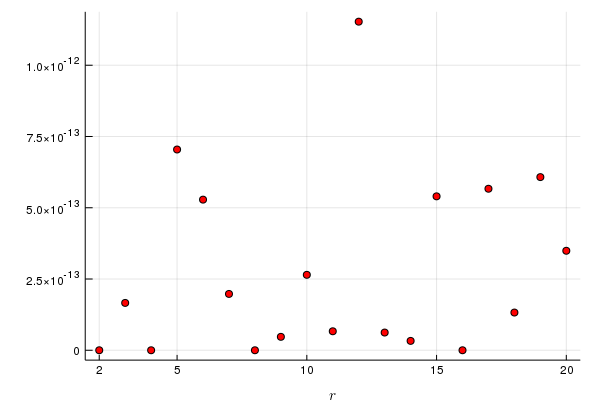
\includegraphics[width=14cm]{error_Czebyszew_to_binomial.png}
\end{figure}
\begin{center}
Maksymalny błąd względny obliczenia współczynnika wielomianu dla danego $r$ i współczynników $A_i$ rzędu liczb naturalnych do 11
\end{center}
Na podstawie powyższego wykresu można poczynić kilka obserwacji. Po pierwsze obliczenia są najdokładniejsze, gdy r jest potęgą dwójki, co może tłumaczyć brak błędów numerycznych w teście pierwszym. Po drugie błędy względne (poza jednym) mieszczą się w przedziale $\left[0, 10^{-12} \right]$.\\

W teście piątym również pojawiły się błędy numeryczne związane z użyciem liczb niecałkowitych. Jednak, jak widać na rycinie na następnej stronie, poprzez fakt, że współczynniki są w tym teście bardzo małe, błąd względny zmalał do wielkości porównywalnych z dokładnością arytmetyki. Widać więc, że dokładność wyniku jest na tyle duża, na ile tylko pozwala implementacja liczb zmiennoprzecinkowych.

\begin{figure}[h!]
  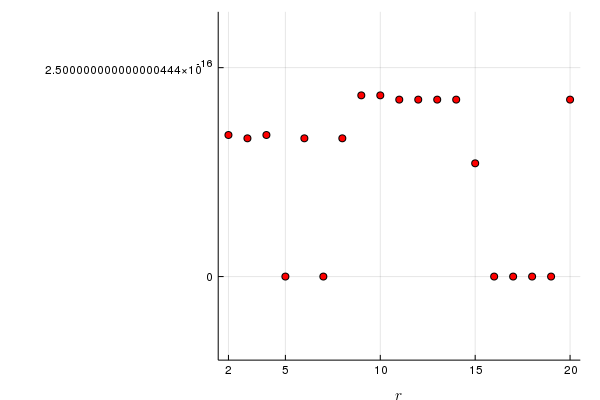
\includegraphics[width=14cm]{error2_Czebyszew_to_binomial.png}
\end{figure}
\newpage
\begin{center}
Maksymalny błąd względny obliczenia współczynnika wielomianu dla danego $r$ i niewielkich współczynników $A_i$
\end{center}
\hfill
\hfill
\hfill

\Large
\textbf{5.Wnioski}
\normalsize

W mojej pracy przedstawiłem algorytm rozwiązujący zadany problem wraz z jego uzasadnieniem. Algorytm działa w czasie kwadratowym względem długości wielomianu wynikowego, ale złożoność zależności obliczanych wspólczynników od danych wejściowych pozwala postawić hipotezę, że lepsza złożoność jest bardzo trudna, jeśli nie niemożliwa do uzyskania.\\

Jak wynika z przeprowadzonych testów, algorytm  oblicza współczynniki poprawnie i z dużą dokładnością, niezależnie od współczynników i stopnia wielomianu oraz postaci, między którymi jest on konwertowany. Błędy wynikają głównie z niedokładności arytmetyki i są niewielkiego rzędu w porównaniu do wyniku.

\newpage
\begin{thebibliography}{9}
\itemsep2pt

\bibitem{WI} Za Wikipedią: \url{https://pl.wikipedia.org/wiki/Wielomian}

\bibitem{JW} J. Wimp, Computation with Recurrence Relations, Pitman Advanced Publishing Program, Boston, 1984

\end{thebibliography}

\end{document}